\documentclass[../../InformazioneQuantistica.tex]{subfiles}

\begin{document}

\onlyinsubfile{\section{L'effetto Zenone quantistico}}
\subsection{Introduzione}
\lesson{4 \greendot}{7/3/2019}
L'idea dell'effetto Zenone quantistico sta nel fatto che, osservando \textit{ripetutamente} e \textit{frequentemente} una particella quantistica la si può \textit{bloccare} nello stesso stato di partenza.\\

In questa sezione \marginpar{Schema dei paragrafi} ci occuperemo di derivare matematicamente l'effetto, usando solo l'operatore di evoluzione temporale unitaria e il postulato di proiezione di von Neumann, seguendo lo schema riportato in \cite{zeno}. Mostreremo quindi un esempio di sistema che esibisce tale fenomeno, e daremo un cenno a come ciò possa essere esito di una \textit{interazione} con l'ambiente, dando un significato \q{più fisico} alle proiezioni geometriche finora usate.\\
Introdurremo poi il concetto di \q{Hamiltoniana} non-hermitiana, che useremo per modellizzare le proiezioni alla von Neumann. Ricondurremo infine tale matrice alla normale Hamiltoniana hermitiana di un sistema considerato \q{non nella sua interezza} (di cui per esempio solo alcuni stati sono di interesse o accessibili - come nel caso di un qubit posto in un apparato complesso).

\subsection{Derivazione dell'Effetto Zenone}
L'evoluzione di un sistema quantistico \textbf{instabile} segue qualitativamente l'andamento riportato in figura \ref{fig:evoluzione-decadimento}.

\begin{figure}[H]
\centering
\includegraphics[width=10.5cm]{Immagini/7_3/image002.png}
\caption{Evoluzione temporale di un sistema quantistico instabile. Sull'asse $y$ è riportata la \textit{survival probability}, ossia la probabilità che il sistema rimanga nello stato iniziale (instabile)\label{fig:evoluzione-decadimento}}
\end{figure}

La probabilità che il sistema rimanga nello stato iniziale esibisce una decrescita quadratica per tempi brevi, che diviene poi esponenziale per tempi medi, e con un andamento in potenza per tempi lunghi. Per l'effetto Zeno ci interessa esaminare nel dettaglio l'andamento quadratico iniziale.\\

Consideriamo allora un sistema isolato inizialmente nello stato $\ket{\psi_0}$ a $t=0$. Poniamo, da qui in avanti, $\hbar=1$ per alleggerire la notazione.\\
AD un certo tempo $t$, il sistema si è evoluto ad uno stato $\ket{\psi(t)}$, che si ottiene dalla formula per l'\textbf{evoluzione unitaria}:
\begin{align}
\ket{\psi(t)} = e^{-iHt}\ket{\psi_0}
\label{eqn:ev-temp}
\end{align}
Ci interessa quantificare quanto $\ket{\psi(t)}$ sia \q{vicino} allo stato iniziale $\ket{\psi_0}$. Consideriamo allora l'\textit{ampiezza} della funzione d'onda che è rimasta \textit{parallela} a $\ket{\psi_0}$, e che è data dal prodotto scalare:
\begin{align}
\mathcal{A}(t) = \braket{\psi_0|\psi(t)} = \bra{\psi_0}e^{-iHt}\ket{\psi_0}
\label{eqn:surv-amplitude}
\end{align}
Prendendo il modulo quadro otteniamo la \textit{probabilità} $p(t)$ che lo stato al tempo $t$ sia ancora pari a quello iniziale, detta \textbf{survival probability}\index{Effetto Zenone!Survival probability}:
\begin{align}
p(t) = |\mathcal{A}(t)|^2 = |\bra{\psi_0}e^{-iHt}\ket{\psi_0}|^2
\label{eqn:surv-prob}
\end{align}
che è pari a $0$ se a $t$ il sistema si trova in uno stato $\ket{\psi(t)}$ \textit{ortogonale} a quello iniziale.\\

Esaminiamo l'evoluzione temporale per un piccolo intervallo di tempo $\delta t$. Sviluppando in serie di MacLaurin la (\ref{eqn:ev-temp}) attorno a $\delta t=0$ si ottiene:
\begin{align*}
\ket{\psi(\delta t)} = e^{-iH\delta t} \ket{\psi_0} \approx \left(\bb{I} - iH\delta t -\frac{H^2}{2} (\delta t)^2 + O((\delta t)^3) \right) \ket{\psi_0} \equiv \ket{\psi_0} + \ket{\delta \psi}
\end{align*}
Tronchiamo questa espressione al secondo ordine, e calcoliamo la \q{survival amplitude} $\mathcal{A}(t)$ prendendo il prodotto scalare con $\ket{\psi_0}$, e riconoscendo i valor medi $\langle H \rangle_{\psi_0}=\bra{\psi_0}H\ket{\psi_0}$:
\begin{align*}
\mathcal{A}(\delta t) = 1 - i\langle H \rangle_{\psi_0} \delta t- \frac{1}{2}\langle H^2 \rangle_{\psi_0} (\delta t)^2
\end{align*}
E a sua volta calcoliamo la survival probability prendendo il modulo quadro, sfruttando il fatto che, poiché $H$ è hermitiano, i suoi valori medi sono reali:\marginpar{Survival probability per tempi piccoli}
\begin{align}\nonumber
p(\delta t) &= \left(1 + i\langle H \rangle_{\psi_0} \delta t- \frac{1}{2}\langle H^2\rangle_{\psi_0} (\delta t)^2 \right) \left(1-i\langle H \rangle_{\psi_0}\delta t - \frac{1}{2}\langle H^2\rangle_{\psi_0}(\delta t)^2\right) \\ \nonumber
&\underset{(a)}{\approx} 1 - \cancel{i\langle H \rangle_{\psi_0} \delta t}- \frac{1}{2}\langle H^2\rangle_{\psi_0} (\delta t)^2 + \cancel{i\langle H \rangle_{\psi_0} \delta t} + \langle H^2\rangle_{\psi_0} (\delta t)^2 - \frac{1}{2}\langle H^2\rangle_{\psi_0} (\delta t)^2=\\
&= 1-(\langle H^2\rangle_{\psi_0} (\delta t)^2 - \langle H^2\rangle_{\psi_0}(\delta t)^2)
= 1-(\delta t)^2 \underbrace{(\langle H^2\rangle_{\psi_0}-\langle H^2\rangle_{\psi_0})}_{\tau_z^{-2}} \equiv 1-\frac{(\delta t)^2}{\tau^2_z} 
\label{eqn:p-tau}
\end{align}
dove in (a) trascuriamo tutti i termini di ordine superiore a $2$. Nell'ultimo passaggio abbiamo introdotto la grandezza $\tau_z$, detta \textbf{tempo di Zenone}\index{Effetto Zenone!Tempo di Zenone}, definita da:
\begin{align}
\tau_z^{-2} \equiv \langle H^2\rangle_{\psi_0} - \langle H \rangle_{\psi_0}^2
\label{eqn:zeno-time}
\end{align}
Dalle espressioni appena ottenute abbiamo che la funzione d'onda evolve \textbf{linearmente} per tempi piccoli\footnote{Su tempi lunghi si osserva invece un'evoluzione esponenziale, che poi si stabilizza in una potenza $t^{-\alpha}$.}, mentre la survival probability \textbf{quadraticamente} in $\delta t$.\\
Abbiamo allora trovato che, almeno per tempi piccoli, un sistema quantistico evolve \q{lentamente}, cioè in modo polinomiale. Ci aspettiamo quindi che, entro un $\delta t$, il sistema sia in uno stato \textit{molto simile} al $\ket{\psi_0}$ iniziale.\\

Dal \textbf{postulato di proiezione di von Neumann} sappiamo che una misura (ideale di prima specie) \textit{proietta} il sistema nell'autostato compatibile con l'esito ottenuto dalla misura. A seguito di tale processo, strettamente \textbf{non unitario}, il nuovo stato riprende ad evolversi in modo unitario. In un certo senso, la misura \q{resetta} l'evoluzione del sistema - dato che in quell'attimo il sistema \textit{non è isolato}.\\

Consideriamo allora una misura che verifichi se il sistema si trova ancora nello stato iniziale $\ket{\psi}$. Ripetiamo tale misura $N$ volte in un tempo $t$, in modo che l'intervallo $\tau$ tra ogni misura sia \textit{molto piccolo}:
\begin{align}
\tau = \frac{t}{N} = \delta t\label{eqn:tau}
\end{align}
Dopo ogni misura il sistema ha una probabilità $p(\tau)$ (survival probability valutata in $t=\tau$) di rimanere nello stato iniziale, e una probabilità $1-p(\tau)$ di muoversi allo stato $\ket{\psi_0^\perp}$ ortogonale a quello iniziale. Se $\tau$ è piccolo, poiché $p(\tau) = 1-\tau^2/\tau_z^2$, avremo $p(\tau) \approx 1$, e perciò il sistema \textit{tende} a rimanere nello stato iniziale.\\

Dopo $N$ misure le probabilità si combinano tra loro\footnote{Stiamo qui trascurando tutti i \textit{percorsi molto improbabili} in cui il sistema visita stati differenti, come quello ortogonale, e poi ritorna a $\ket{\psi}_0$ nel corso delle $N$ misure.}, e si ha $\ket{\psi(t)}=\ket{\psi_0}$ con una probabilità:
\begin{align*}
p^{(N)}(t) = \left[p(\tau)\right]^N \underset{(\ref{eqn:p-tau})}{=} \left[1-\frac{\tau^2}{\tau_z^2}\right]^N \underset{(\ref{eqn:tau})}{=} \left(1-\left(\frac{t}{N \tau_z}\right)^2\right)^N \xrightarrow[(b)]{N \gg 1} \exp\left(-\frac{t^2}{N\tau_z^2}\right) \xrightarrow[{N\to\infty}]{}1
\end{align*}
dove in (b) si è usata la definizione dell'esponenziale:
\begin{align*}
e^x = \lim_{n\to+\infty} \left(1+\frac{x}{n}\right)^n
\end{align*}
Perciò, al limite di \textit{misure infinitamente frequenti}, l'evoluzione del sistema in esame è \textbf{completamente arrestata}.

\begin{figure}[H]
\centering
%\includegraphics[width=10.5cm]{Immagini/7_3/image001.png}


\tikzset{every picture/.style={line width=0.75pt}} %set default line width to 0.75pt        
\begin{center}
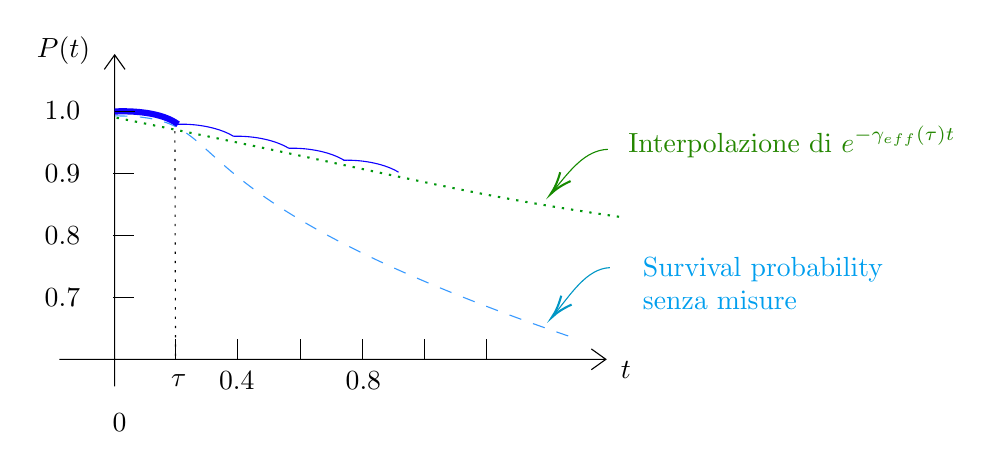
\begin{tikzpicture}[x=0.75pt,y=0.75pt,yscale=-1,xscale=1]
%uncomment if require: \path (0,300); %set diagram left start at 0, and has height of 300

%Shape: Axis 2D [id:dp21522982327423357] 
\draw  (121,175.67) -- (384.33,175.67)(147.67,29) -- (147.67,188.67) (377.33,170.67) -- (384.33,175.67) -- (377.33,180.67) (142.67,36) -- (147.67,29) -- (152.67,36)  ;
%Curve Lines [id:da15785243874113397] 
\draw [color={rgb, 255:red, 57; green, 154; blue, 255 }  ,draw opacity=1 ] [dash pattern={on 4.5pt off 4.5pt}]  (147.84,58.4) .. controls (211.43,58.4) and (159.31,93.88) .. (370.38,165.86) ;


%Curve Lines [id:da8350402313780105] 
\draw [color={rgb, 255:red, 15; green, 0; blue, 255 }  ,draw opacity=1 ][line width=2.25]    (147.68,56.27) .. controls (156.47,55.9) and (170.29,56.57) .. (178.23,62.42) ;


%Curve Lines [id:da6358485219303893] 
\draw [color={rgb, 255:red, 15; green, 0; blue, 255 }  ,draw opacity=1 ]   (178.23,62.42) .. controls (188.78,62.12) and (199,64.56) .. (204.88,68.21) ;


%Curve Lines [id:da4404463330552182] 
\draw [color={rgb, 255:red, 15; green, 0; blue, 255 }  ,draw opacity=1 ]   (204.88,68.21) .. controls (215.43,67.91) and (225.64,70.34) .. (231.53,73.99) ;


%Curve Lines [id:da9745888558673619] 
\draw [color={rgb, 255:red, 15; green, 0; blue, 255 }  ,draw opacity=1 ]   (231.53,73.99) .. controls (242.07,73.69) and (252.29,76.12) .. (258.17,79.77) ;


%Curve Lines [id:da3527462322133508] 
\draw [color={rgb, 255:red, 15; green, 0; blue, 255 }  ,draw opacity=1 ]   (257.81,79.76) .. controls (268.36,79.46) and (278.58,81.89) .. (284.46,85.54) ;


%Straight Lines [id:da34568675396501636] 
\draw  [dash pattern={on 0.84pt off 2.51pt}]  (176.69,65.72) -- (177,176) ;


%Curve Lines [id:da052117335217273464] 
\draw [color={rgb, 255:red, 0; green, 150; blue, 12 }  ,draw opacity=1 ][line width=0.75]  [dash pattern={on 0.84pt off 2.51pt}]  (148.61,59.31) .. controls (287.18,87.19) and (313.34,95.81) .. (391.17,107.06) ;


%Straight Lines [id:da6118859076103123] 
\draw    (147,146) -- (157,146) ;


%Straight Lines [id:da17183505389897635] 
\draw    (147,116) -- (157,116) ;


%Straight Lines [id:da4284019112663999] 
\draw    (147,86) -- (157,86) ;


%Straight Lines [id:da2724371012042419] 
\draw    (147.68,56.27) -- (157.68,56.27) ;


%Straight Lines [id:da45937983782048275] 
\draw    (237,176) -- (237,166) ;


%Straight Lines [id:da9979635498053909] 
\draw    (207,176) -- (207,166) ;


%Straight Lines [id:da7060313167766665] 
\draw    (177,176) -- (177,166) ;


%Straight Lines [id:da27852080941520097] 
\draw    (267,176) -- (267,166) ;


%Straight Lines [id:da4124681634033196] 
\draw    (297,176) -- (297,166) ;


%Straight Lines [id:da7767131492541457] 
\draw    (327,176) -- (327,166) ;


%Curve Lines [id:da4361033074713996] 
\draw [color={rgb, 255:red, 22; green, 138; blue, 0 }  ,draw opacity=1 ]   (385.25,74.5) .. controls (374.09,74.97) and (366.99,84.93) .. (359.02,94.49) ;
\draw [shift={(357.75,96)}, rotate = 310.36] [color={rgb, 255:red, 22; green, 138; blue, 0 }  ,draw opacity=1 ][line width=0.75]    (10.93,-3.29) .. controls (6.95,-1.4) and (3.31,-0.3) .. (0,0) .. controls (3.31,0.3) and (6.95,1.4) .. (10.93,3.29)   ;

%Curve Lines [id:da44210673825584834] 
\draw [color={rgb, 255:red, 0; green, 150; blue, 197 }  ,draw opacity=1 ]   (386.25,131.5) .. controls (375.09,131.98) and (367.54,144.18) .. (359.52,153.98) ;
\draw [shift={(358.25,155.5)}, rotate = 310.36] [color={rgb, 255:red, 0; green, 150; blue, 197 }  ,draw opacity=1 ][line width=0.75]    (10.93,-3.29) .. controls (6.95,-1.4) and (3.31,-0.3) .. (0,0) .. controls (3.31,0.3) and (6.95,1.4) .. (10.93,3.29)   ;


% Text Node
\draw (122.5,56) node   {$1.0$};
% Text Node
\draw (122.5,86) node   {$0.9$};
% Text Node
\draw (122.5,116) node   {$0.8$};
% Text Node
\draw (122.5,146) node   {$0.7$};
% Text Node
\draw (150,206) node   {$0$};
% Text Node
\draw (178.5,186) node   {$\tau $};
% Text Node
\draw (206.5,186) node   {$0.4$};
% Text Node
\draw (267.5,186) node   {$0.8$};
% Text Node
\draw (460,139) node [color={rgb, 255:red, 0; green, 158; blue, 238 }  ,opacity=1 ] [align=left] {Survival probability\\senza misure};
% Text Node
\draw (474,71) node [color={rgb, 255:red, 36; green, 134; blue, 0 }  ,opacity=1 ] [align=left] {Interpolazione di $\displaystyle e^{-\gamma _{\text{eff}}( \tau ) t}$};
% Text Node
\draw (394,181) node   {$t$};
% Text Node
\draw (123,27) node   {$P( t)$};


\end{tikzpicture}
\end{center}
\caption{Effetto di Zeno quantistico per $N=5$ misure \q{alla Von Neumann}. La linea blu continua mostra la \textit{survival probability} nel caso di misure ripetute, mentre quella azzurra tratteggiata nel caso \textit{senza misure}. La linea in verde puntinata è l'esponenziale che \textit{interpola} l'effetto Zeno definito in (\ref{eqn:Zeno-exp}).\label{fig:effetto-Zeno}}
\end{figure}

La \textit{survival probability} dopo $N$ misure può essere interpolata da un'esponenziale:
\begin{align}
p^{(N)}(t) = p(\tau)^N = \exp(N\log p(\tau)) \underset{N=t/\tau}{=} \exp\left(t \frac{\log p(\tau)}{\tau}\right) = \exp(-\gamma_{\op{eff}}(\tau)t)
\label{eqn:Zeno-exp}
\end{align}
dove abbiamo definito opportunamente la \q{costante di decadimento effettiva} $\gamma_{\op{eff}}$ come:
\begin{align*}
\gamma_{\op{eff}} = -\frac{1}{\tau}\log p(\tau)
\end{align*}
Per $\tau \to 0$, che corrisponde a $N\to \infty$, vale l'espansione $p(\tau)=1-\tau^2/\tau_z^2$, e quindi ricaviamo:
\begin{align}
\gamma_{\op{eff}}(\tau) \approx \frac{\tau}{\tau_z^2}\qquad \tau \to 0
\label{eqn:gamma-eff}
\end{align}

Riepilogando, se si esegue una misure ogni $\tau$, la probabilità $p(t)$ che il sistema rimanga nello stato iniziale $\ket{\psi_0}$ ha l'andamento esponenziale decrescente della frazione \textit{non decaduta} di atomi radioattivi. Il decadimento è tanto più lento quanto $\gamma_{\op{eff}}$, proporzionale a $\tau$, è piccolo. Perciò, nell'ipotetico caso in cui si effettui una misura ad ogni istante, $\tau=0$, $\gamma_{\op{eff}}=\infty$ e $p(t)\equiv 1 \> \forall t$.

\subsection{Esempio di effetto Zenone}
Un \textit{caso semplice} che possiamo usare per studiare l'effetto Zenone è dato da un sistema che effettua \textit{oscillazioni di Rabi}.\index{Esempio!Effetto Zenone per oscillazioni di Rabi}\index{Effetto Zenone!Oscillazioni di Rabi} Possiamo immaginarlo come un atomo con due livelli a energia diversa, che viene illuminato da un raggio di fotoni di energia (definita dalla loro \textit{frequenza}) pari a quella di transizione tra i due livelli. Si osserva che il sistema \textit{oscilla} tra i due stati: prima assorbe un fotone per portarsi al livello eccitato, e poi ritorna indietro per \textit{emissione stimolata} (analogamente a quanto avviene in un laser).\\

Detti $\ket{0}$ e $\ket{1}$ gli stati corrispondenti ai due livelli, nella base $\{\ket{0},\ket{1}\}$ l'Hamiltoniana di un sistema del genere diviene:
\begin{align}
H = \Omega \hat{\sigma}_x = \begin{pmatrix}0 & \Omega\\\Omega & 0\end{pmatrix} \qquad \ket{\psi_0}=\ket{0}
\label{eqn:rabi-oscillation-H}
\end{align}
dove i termini fuori dalla diagonale sono indicativi degli \textit{accoppiamenti} (\textit{coupling}) tra livelli, ossia delle probabilità di transizione tra $\ket{0}$ e $\ket{1}$ e viceversa.\\

\textbf{Nota}: poiché vogliamo descrivere un sistema che oscilla (per evoluzione unitaria) tra due stati $\ket{0}$ e $\ket{1}$, si ha che tali $\ket{0}$ e $\ket{1}$ \textbf{non} possono essere autoket di $H$: se lo fossero sarebbero stati stazionari, e non sarebbe possibile un'evoluzione da uno all'altro senza un disturbo esterno.\\
Infatti, se $\ket{0}$ è autoket di $H$, l'equazione di Schr\"odinger dipendente dal tempo ha come soluzione un'onda stazionaria che resta in $\ket{0}$:
\begin{align*}
i\hbar \frac{\partial}{\partial t} \ket{0} =\mathcal{E}_0 \ket{0}\Rightarrow \ket{\psi(t)}=e^{-i\mathcal{E}_0t}\ket{0}
\end{align*}
Segue che, scrivendo $H$ in una base $\{\ket{0},\ket{1}\}$ che \textbf{non} è costituita dai suoi autoket, $H$ \textit{non può essere diagonale}.\\

L'evoluzione temporale determinata da $H$ è data da:
\begin{align*}
\ket{\psi(t)} = e^{-iHt} \ket{\psi_0} = \exp\left(-i\Omega t\begin{pmatrix}
0 & 1\\1 & 0\end{pmatrix}\right) \begin{pmatrix} 1 \\ 0 \end{pmatrix}
\end{align*}
L'esponenziale di matrice si calcola in modo diretto notando che:
\begin{align*}
A=\begin{pmatrix}0 & 1\\1 & 0\end{pmatrix}; \qquad A^2 = \bb{I}
\end{align*}
Da cui:
\begin{align*}
\exp(-i\Omega t A) &= 1 +(-i\Omega t)A + \frac{1}{2!}(-i\Omega t)^2 \bb{I} + \frac{1}{3!}(-i\Omega t)^3 A + \dots =\\
&= 1 +(-i)[\Omega t] A -\frac{1}{2!}[\Omega t]^2 \bb{I} - \frac{1}{3!}(-i)[\Omega t]^3 A +\dots =\\
&=\bb{I}\sum_{k=0}^{+\infty} (-1)^k \frac{(\Omega t)^{2k}}{(2k)!} + (-i)A \sum_{k=0}^{+\infty} (-1)^k \frac{(\Omega t)^{2k+1}}{(2k+1)!}=\\ &= \bb{I}\cos(\Omega t)-iA\sin(\Omega t) = \begin{pmatrix}
\cos(\Omega t) & -i\sin(\Omega t)\\
-i\sin(\Omega t) & \cos(\Omega t)\end{pmatrix}
\end{align*}
Moltiplicando per $\ket{\psi_0}=\ket{0}=(1,0)^T$ otteniamo allora:
\begin{align*}
\ket{\psi(t)}=\cos(\Omega t)\ket{0} -i\sin(\Omega t)\ket{1}
\end{align*}
Calcoliamo quindi $\mathcal{A}(t)$ e $p(t)$ tramite (\ref{eqn:surv-amplitude}) e (\ref{eqn:surv-prob}):
\begin{align*}
\mathcal{A}(t) &= \braket{\psi_0|\psi(t)}= \cos(\Omega t)\\
\Rightarrow p(t) &= |\mathcal{A}(t)|^2 =\cos^2 (\Omega t) = 1 - [\Omega t]^2 + \frac{[\Omega t]^3}{3!} + O([\Omega t]^6)
\end{align*}
Per il tempo di Zenone usiamo la definizione (\ref{eqn:zeno-time}):
\begin{align*}
\tau_z^{-2} = \langle H^2 \rangle_{\psi_0}-\langle H \rangle_{\psi_0}^2
\end{align*}
dove il calcolo del valor medio, in notazione matriciale, diviene:
\begin{align*}
\langle H\rangle_{\psi_0} &= \bra{0}H\ket{0} = \begin{pmatrix}1 & 0\end{pmatrix}\begin{pmatrix} 0 & \Omega\\\Omega & 0\end{pmatrix}\begin{pmatrix}1 \\ 0\end{pmatrix}=0\\
\langle H^2 \rangle_{\psi_0} &= \bra{0}H^2\ket{0}\ = \begin{pmatrix} 1 & 0\end{pmatrix}\begin{pmatrix} \Omega^2 & 0\\ 0 & \Omega^2 \end{pmatrix}\begin{pmatrix} 1 \\ 0\end{pmatrix}=\Omega^2
\end{align*}
E otteniamo:
\begin{align}
\tau_z^{-2}=\Omega^2 \Rightarrow \tau_z=\Omega^{-1};\qquad \gamma_{\op{eff}} \underset{(\ref{eqn:gamma-eff})}{=}\tau \Omega^2\label{eqn:gamma-eff-esempio}  
\end{align}
Notiamo in particolare che vale l'espansione da cui abbiamo ricavato il tempo di Zenone:
\begin{align*}
p(t) \approx 1 - \frac{t^2}{\tau_z^2} = 1-\Omega^2 t^2
\end{align*}

\subsection{Effetto Zenone per interazione}
Nel calcolare il tempo di Zenone $\tau_z$ nell'esempio abbiamo visto, si è trovato che l'unico contributo deriva da $\langle H^2 \rangle_{\psi_0}$. Questo \textit{non} è un caso, ma è indice dell'origine dell'effetto Zenone come \textit{interazione}.\\
In generale, consideriamo un sistema di Hamiltoniana $H$, che dividiamo in una matrice diagonale $H_0$ e una matrice con tutti gli elementi che non stanno sulla diagonale $H_{\op{int}}$ che indica i \textit{coupling} tra i livelli energetici, e quindi chiamiamo \textbf{hamiltoniana di interazione}.\index{Effetto Zenone!Hamiltoniana di interazione}
%Esattamente che base stiamo usando prima di scomporre l'Hamiltoniana in free e interaction?
\begin{align*}
H=H_0+ H_{\op{int}}
\end{align*}
Siano $\{\ket{\psi_n}\}$ gli autostati di $H_0$, e $\ket{\psi_0}$ sia uno di essi:
\begin{align*}
H_0 \ket{\psi_0} = \omega_0 \ket{\psi_0}
\end{align*}
Calcoliamo il tempo di Zenone $\tau_z$ dalla definizione:
\begin{align*}
\tau_z^{-2} = \langle H^2 \rangle_{\psi_0}-\langle H \rangle_{\psi_0} = \langle H_0^2 + H_0 H_{\op{int}} + H_{\op{int}}H_0 + H_{\op{int}}^2 \rangle_{\psi_0}-\langle H_0 + H_{\op{int}}\rangle_{\psi_0}
\end{align*}
Notiamo che $\langle H_{\op{int}}\rangle_{\psi_0} = 0$, dato che il valor medio \q{seleziona} un termine sulla diagonale, che è nulla per come abbiamo definito $H_{\op{int}}$. Allo stesso modo, i prodotti tra $H_0$ e $H_{\op{int}}$ hanno sempre la diagonale nulla. Infatti moltiplicando una matrice diagonale $A$ con una $B$ con diagonale nulla si ottiene una matrice $C$ con diagonale nulla:
\begin{align*}
C_{ij} = A_{ik}B_{kj}=\delta_{ik}A_{ik}B_{kj}\Rightarrow C_{ii}=A_{ii}B_{ii}=0
\end{align*}
Perciò i valor medi dei \q{termini misti} sono nulli. Inoltre, dato che $\ket{\psi_0}$ è autostato di $H_0$ vale (per definizione di autostato):
\begin{align*}
\langle H_0^2 \rangle_{\psi_0} - \langle H_0 \rangle^2_{\psi_0} =0
\end{align*}  
Perciò resta un unico termine:
\begin{align*}
\tau_z^{-2} = \langle H_{\op{int}}^2 \rangle_{\psi_0} = \sum_n \bra{\psi_0}H_{\op{int}}\ket{\psi_n}\bra{\psi_n}H_{\op{int}}\ket{\psi_0}
\end{align*}
Perciò, in questo caso il tempo di Zenone dipende esclusivamente dall'Hamiltoniana di interazione, che contiene i \textit{coupling} tra i livelli del sistema considerato. Come vedremo nei prossimi paragrafi, questa idea di \textit{interazione} sorge esaminando nel dettaglio i \q{retroscena} delle proiezioni di Von Neumann.

\subsection{Matrici \q{Hamiltoniane} non hermitiane}

Poiché l'operatore $U$ di evoluzione temporale è unitario, si ha che:
\begin{align*}
\braket{\psi(t)|\psi(t)} = \braket{\psi_0|\psi_0}
\end{align*} 
Perciò l'evoluzione temporale di un qubit avviene tra punti posti sulla \textit{superficie} della sfera di Bloch, ossia rimane nel sottospazio di Hilbert definito da $\norm{\psi}=1$ (figura \ref{fig:sfera-bloch-evoluzione}.a). Un'eventuale evoluzione non unitaria (figura \ref{fig:sfera-bloch-evoluzione}.b) fa sì che la funzione d'onda \textit{abbandoni} tale sottospazio (come vedremo più in dettaglio nelle prossime sezioni).

\begin{figure}[H]
\centering
%\includegraphics[width=10.5cm]{Immagini/7_3/image003.png}


\tikzset{every picture/.style={line width=0.75pt}} %set default line width to 0.75pt        
\begin{center}
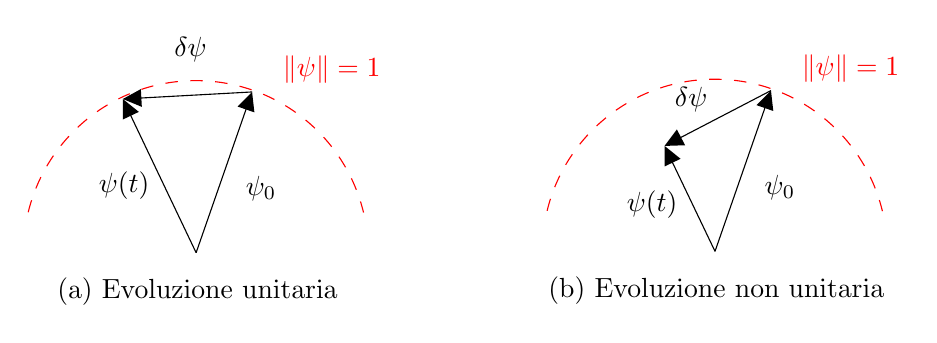
\begin{tikzpicture}[x=0.75pt,y=0.75pt,yscale=-1,xscale=1]
%uncomment if require: \path (0,300); %set diagram left start at 0, and has height of 300

%Straight Lines [id:da13244260408452746] 
\draw    (192.71,166.46) -- (219.01,90.89) ;
\draw [shift={(219.67,89)}, rotate = 469.19] [fill={rgb, 255:red, 0; green, 0; blue, 0 }  ][line width=0.75]  [draw opacity=0] (8.93,-4.29) -- (0,0) -- (8.93,4.29) -- cycle    ;

%Shape: Arc [id:dp47261095341946513] 
\draw  [draw opacity=0][dash pattern={on 4.5pt off 4.5pt}] (111.82,146.94) .. controls (120.55,110.84) and (152.96,83.88) .. (191.85,83.54) .. controls (231.29,83.2) and (264.56,110.36) .. (273.36,147.09) -- (192.57,166.46) -- cycle ; \draw  [color={rgb, 255:red, 255; green, 0; blue, 0 }  ,draw opacity=1 ][dash pattern={on 4.5pt off 4.5pt}] (111.82,146.94) .. controls (120.55,110.84) and (152.96,83.88) .. (191.85,83.54) .. controls (231.29,83.2) and (264.56,110.36) .. (273.36,147.09) ;
%Straight Lines [id:da4640817340211536] 
\draw    (192.71,166.46) -- (158.26,94.2) ;
\draw [shift={(157.4,92.39)}, rotate = 424.51] [fill={rgb, 255:red, 0; green, 0; blue, 0 }  ][line width=0.75]  [draw opacity=0] (8.93,-4.29) -- (0,0) -- (8.93,4.29) -- cycle    ;

%Straight Lines [id:da676932203344851] 
\draw    (219.67,89) -- (159.4,92.29) ;
\draw [shift={(157.4,92.39)}, rotate = 356.88] [fill={rgb, 255:red, 0; green, 0; blue, 0 }  ][line width=0.75]  [draw opacity=0] (8.93,-4.29) -- (0,0) -- (8.93,4.29) -- cycle    ;

%Straight Lines [id:da439787380235227] 
\draw    (442.71,165.79) -- (469.01,90.22) ;
\draw [shift={(469.67,88.33)}, rotate = 469.19] [fill={rgb, 255:red, 0; green, 0; blue, 0 }  ][line width=0.75]  [draw opacity=0] (8.93,-4.29) -- (0,0) -- (8.93,4.29) -- cycle    ;

%Shape: Arc [id:dp10305939137664444] 
\draw  [draw opacity=0][dash pattern={on 4.5pt off 4.5pt}] (361.82,146.27) .. controls (370.55,110.17) and (402.96,83.21) .. (441.85,82.87) .. controls (481.29,82.53) and (514.56,109.69) .. (523.36,146.43) -- (442.57,165.79) -- cycle ; \draw  [color={rgb, 255:red, 255; green, 0; blue, 0 }  ,draw opacity=1 ][dash pattern={on 4.5pt off 4.5pt}] (361.82,146.27) .. controls (370.55,110.17) and (402.96,83.21) .. (441.85,82.87) .. controls (481.29,82.53) and (514.56,109.69) .. (523.36,146.43) ;
%Straight Lines [id:da4447134676498914] 
\draw    (442.71,165.79) -- (419.26,116.8) ;
\draw [shift={(418.4,115)}, rotate = 424.41999999999996] [fill={rgb, 255:red, 0; green, 0; blue, 0 }  ][line width=0.75]  [draw opacity=0] (8.93,-4.29) -- (0,0) -- (8.93,4.29) -- cycle    ;

%Straight Lines [id:da8691059971533945] 
\draw    (469.67,88.33) -- (420.17,114.08) ;
\draw [shift={(418.4,115)}, rotate = 332.52] [fill={rgb, 255:red, 0; green, 0; blue, 0 }  ][line width=0.75]  [draw opacity=0] (8.93,-4.29) -- (0,0) -- (8.93,4.29) -- cycle    ;


% Text Node
\draw (158,134) node   {$\psi ( t)$};
% Text Node
\draw (224,135.6) node   {$\psi _{0}$};
% Text Node
\draw (190,68.4) node   {$\delta \psi $};
% Text Node
\draw (258,78.2) node [color={rgb, 255:red, 255; green, 0; blue, 0 }  ,opacity=1 ]  {$\| \psi \| =1$};
% Text Node
\draw (193.33,185.33) node  [align=left] {(a) Evoluzione unitaria};
% Text Node
\draw (412.4,143.33) node   {$\psi ( t)$};
% Text Node
\draw (474,134.93) node   {$\psi _{0}$};
% Text Node
\draw (431.2,92.8) node   {$\delta \psi $};
% Text Node
\draw (508,77.53) node [color={rgb, 255:red, 255; green, 0; blue, 0 }  ,opacity=1 ]  {$\| \psi \| =1$};
% Text Node
\draw (443.33,184.67) node  [align=left] {(b) Evoluzione non unitaria};


\end{tikzpicture}
\end{center}
\caption{L'evoluzione unitaria (a) fa sì che un vettore non abbandoni mai la superficie della sfera di Bloch, cosa che invece succede nel caso non unitario (b).\label{fig:sfera-bloch-evoluzione}}
\end{figure}

L'evoluzione di sistemi instabili, in cui la \textit{survival probability} diminuisce nel tempo, può essere vista come un processo che \q{porta via probabilità}, ossia un'evoluzione non unitaria. In altre parole, ci stiamo muovendo nella direzione di \textit{integrare} gli effetti delle misure ripetute precedentemente considerate direttamente nell'Hamiltoniana.\\

Per trattare l'evoluzione non unitaria si introduciamo allora \textit{ad hoc} una \q{Hamiltoniana modificata} data da:
\begin{align}
H = H -i V\bb{I} \qquad V\in \bb{R}^+
\label{eqn:non-hermitian-Hamiltonian}
\end{align} 
dove $V$ è un'opportuna grandezza detta \textbf{potenziale ottico}\footnote{In maniera pittoresca, si può pensare all'evoluzione della funzione d'onda come a quella della luce che si propaga in un mezzo \textit{rifrattivo} e \textit{dissipativo}. Da qui l'idea di aggiungere un \q{potenziale ottico} per tenere conto di tali \q{dissipazioni di probabilità}.}\index{Potenziale ottico}\index{Effetto Zenone:Hamiltoniane non hermitiane}.\\
Un sistema che evolve con un'Hamiltoniana del genere, che non è hermitiana, \q{perde probabilità}, ossia giunge a stati non normalizzati. Partendo da uno stato iniziale $\ket{\psi_0}$, avremo cioè $\norm{\ket{\psi(t)}} \leq \norm{\ket{\psi_0}}$. Fisicamente, tale \q{probabilità mancante} va a finire in altri stati - non contemplati nel sistema che stiamo esaminando - attraverso un \textit{decay channel}. Pittorescamente, possiamo immaginare la probabilità come un fluido, racchiuso in un contenitore, di cui osserviamo la dinamica. L'evoluzione unitaria corrisponde allora alla \textit{visuale completa} dell'intero contenitore, per cui la \textit{quantità di fluido} osservata rimane sempre la stessa. Se invece ci concentriamo solo su una parte dell'insieme, può capitare che del fluido scorra via, muovendosi nel resto del sistema, e apparentemente scomparendo da questa visuale \textit{parziale}.\\
Giustificheremo tutto ciò matematicamente tra qualche paragrafo. Per ora, partiamo analizzando l'evoluzione dettata dall'Hamiltoniana non hermitiana appena introdotta, calcolandone \textit{survival amplitude} $\mathcal{A}(t)$ e \textit{survival probability} $p(t)$:
\begin{align*}
\mathcal{A}(\delta t) &= e^{-Vt} \bra{\psi_0} e^{-iH\delta t}\ket{\psi_0}=\\
&=\left(1-V\delta t + \frac{1}{2}V^2 [\delta t]^2 + O([\delta t]^3)\right)\left[1 - i\langle H \rangle_{\psi_0}\delta t-\frac{1}{2}\langle H^2 \rangle_{\psi_0}[\delta t]^2 + \dots \right]=\\
&= 1-\left(V+i\langle H \rangle_{\psi_0}\right)\delta t -\frac{1}{2}\left(\langle H^2\rangle_{\psi_0} - V^2 - 2iV\langle H \rangle_{\psi_0} \right) [\delta t]^2 + O([\delta t]^3)\\
p(\delta t) &= e^{-2Vt} |\bra{\psi_0} e^{-iHt}\ket{\psi_0}|^2 \approx 1-2V \delta t + O([\delta t]^2)
\end{align*}
Otteniamo perciò un decadimento \textbf{lineare} per tempi piccoli sia per la \textit{survival amplitude} $\mathcal{A}(\delta t)$ che per la \textit{survival probability} $p(\delta t)$.


\subsection{Effetto Zenone senza proiezioni}
All'inizio della trattazione, abbiamo spiegato l'effetto Zenone quantistico in termini di \textit{misure ripetute}, attuate come un rapido susseguirsi di proiezioni di Von Neumann. Ma qual è il \textit{significato fisico} di ciascuna di tale proiezioni?\\
Secondo il parere attuale di diversi fisici, una proiezione di Von Neumann non è altro che una \textit{notazione abbreviata} dell'effetto (idealizzato) del complicato processo che porta alla misurazione, tramite apparati macroscopici, di caratteristiche microscopiche di un sistema. Pur non essendo chiari i dettagli di tale processo (e in effetti si parla di \textit{measurement problem}), possiamo lo stesso cercarne una \textit{descrizione effettiva}.\\
In particolare, possiamo usare le \q{Hamiltoniane} non hermitiane appena introdotte per descrivere l'effetto delle misurazioni, che porta ad un ben preciso andamento della \textit{survival probability}, come osservato.\\

Partiamo allora dall'esempio (\ref{eqn:rabi-oscillation-H}), a cui aggiungiamo un termine non hermitiano $-i2V$, giungendo all'Hamiltoniana (espressa in notazione matriciale nella base $\{\ket{0}, \ket{1}\})$:
\begin{align}
H_{\op{int}} = \begin{pmatrix} 0 & \Omega \\ \Omega & - 2iV\end{pmatrix} = -iV \bb{I} + \vec{h}\cdot \vec{\sigma} \qquad \vec{\sigma} = \begin{pmatrix} \sigma_x\\\sigma_y \\ \sigma_z\end{pmatrix}; \> \vec{h} = \begin{pmatrix} \Omega \\ 0 \\ iV \end{pmatrix}
\label{eqn:H-non-hermitiana-esempio}
\end{align}
Il sistema parte dallo stato iniziale $\ket{0}$ ed evolve verso $\ket{1}$, come visto nell'esempio iniziale. Tuttavia, nella colonna di $\ket{1}$ abbiamo inserito un termine non hermitiano $-i2V$, che non è altro che una versione asimmetrica della modifica già esaminata in (\ref{eqn:non-hermitian-Hamiltonian}), che ha quindi l'effetto di \q{assorbire} la probabilità \textbf{solo} dallo stato $\ket{1}$ verso cui evolve il sistema, e che funge quindi da \q{decay channel}. Ci interessa capire se la \textit{survival probability} $p(t)$ calcolata con una $H_{\op{int}}$ non hermitiana può riprodurre l'andamento \q{esponenziale efficace} dell'effetto Zenone con $N$ proiezioni di Von Neumann ripetute.\\

\textbf{Nota}: Il fattore $2$ presente nel termine non hermitiano serve solo a semplificare i conti, dato che permette una scomposizione di $H_{\op{int}}$ come somma di una matrice identità $\bb{I}$ per un opportuno fattore, e di un \textbf{vettore di Pauli} $\vec{h}\cdot \vec{\sigma}$.\\


Partiamo allora calcolando l'evoluzione temporale del sistema a partire dallo stato $\ket{\psi_0}=\ket{0}$:
\begin{align*}
\ket{\psi(t)} = e^{-iH_{\op{int}}t} \ket{0} = \exp[{-it(-iV\bb{I}+\vec{h}\cdot\vec{\sigma})}] \underset{(a)}{=} \exp(-Vt\bb{I})\exp(-it\vec{h}\cdot \vec{\sigma})
\end{align*}
dove il passaggio in (a) è giustificato dal fatto che $\bb{I}$ commuta con qualsiasi matrice, e in particolare con $\vec{h}\cdot \vec{\sigma}$.\\
Il primo esponenziale si calcola velocemente:
\begin{align*}
\exp(-Vt \bb{I}) = e^{-Vt}\bb{I} 
\end{align*}
Per il secondo, invece, usiamo il risultato:
\begin{align}
e^{i\vec{a}\cdot \vec{\sigma}}=e^{ia(\hat{n}\cdot \vec{\sigma})} = \bb{I}\cos(a) + i(\hat{n}\cdot \vec{\sigma})\sin(a)
\label{eqn:exp-pauli-vector}
\end{align}
dove $\vec{a} \in \bb{C}^3$ è un generico vettore, che fattorizziamo in prodotto di modulo e versore: $\vec{a}=a\hat{n}$, con $\norm{\hat{n}}=1$. Tale formula si dimostra\footnote{Vedi esercizi del corso di Metodi Matematici} notando che $(\hat{n}\cdot \vec{\sigma})^{2k}=\bb{I}$ e $(\hat{n}\cdot \vec{\sigma})^{2k+1}=\hat{n}\cdot\vec{\sigma}$ (con $k\in \bb{Z}$), scrivendo i primi termini dello sviluppo e riconoscendo le espansioni di $\sin$ e $\cos$.\\

Nel nostro caso, partiamo scomponendo $\vec{h}$:
\begin{align*}
\norm{\vec{h}}^2={\vec{h}\cdot\vec{h}}=\Omega^2-V^2
\end{align*}
Per esaminare l'effetto Zenone ci servirà un \textbf{forte coupling} con l'ambiente, ossia\marginpar{Strong coupling} $\bm{V\gg \Omega}$. Perciò possiamo scrivere il modulo di $\vec{h}$ in termini di un'opportuna grandezza $h$, che definiamo positiva per comodità:
\begin{align}
\norm{\vec{h}}=i\sqrt{V^2-\Omega^2}\equiv ih \Rightarrow h=\sqrt{V^2-\Omega^2}>0
\label{eqn:h-def}
\end{align}
Possiamo allora applicare la (\ref{eqn:exp-pauli-vector}) all'esponenziale che dobbiamo calcolare:
\begin{align*}
\exp(-it\vec{h}\cdot \vec{\sigma})&=\exp\left(i\underbrace{(-\textcolor{Blue}{ih}t)}_{a} \underbrace{\frac{\vec{h}}{\textcolor{Blue}{ih}}\cdot \vec{\sigma}}_{\hat{n}\cdot\vec{\sigma}}\right) =
\bb{I}\cos(-iht) + i^2 \left(\frac{\vec{h}\cdot\vec{\sigma}}{ih}\right)\sin(-iht) =\\
&\underset{(a)}{=}\bb{I}\cosh(ht) -i(-i\sin(iht))\left(\frac{\vec{h}\cdot\vec{\sigma}}{h}\right) \underset{(b)}{=} \cosh(ht)\bb{I} - i\sinh(th) \left(\frac{\vec{h}\cdot\vec{\sigma}}{h}\right)
\end{align*}
Dove in (a) e in (b) abbiamo usato rispettivamente le due relazioni:
\begin{align*}
\cos(ix) = \cosh(x) \qquad -i\sin(ix) = \sinh(x)
\end{align*}

Mettendo insieme i due pezzi otteniamo:
\begin{align*}
e^{-iH_{\op{int}}t}=e^{-Vt}\begin{pmatrix}
\cosh(ht) + \frac{V}{h}\sinh(ht) & -i\frac{\Omega}{h}\sinh(ht)\\
-i\frac{\Omega}{h}\sinh(ht) & \cosh(ht) +\frac{V}{h}\sinh(ht)
\end{pmatrix}
\end{align*}

Possiamo ora finalmente calcolare la \textit{survival amplitude} $\mathcal{A}(t)$:
\begin{align*}
\mathcal{A}(t) &= \bra{0}e^{-iH_{\op{int}}t}\ket{0} = e^{-Vt}\left[\cosh(ht) + \frac{V}{h}\sinh(ht)\right]=\\
&\underset{(a)}{=} \frac{1}{2}\left(1+\frac{V}{h}\right) \hlc{Yellow}{e^{-(V-h)t} }+\frac{1}{2}\left(1-\frac{V}{h}\right) \hlc{SkyBlue}{e^{-(V+h)t}}
\end{align*}
dove in (a) abbiamo riscritto le funzioni iperboliche tramite esponenziali ($\sinh(x)=(e^{x}-e^{-x})/2$, $\cosh(x)=(e^{x}+e^{-x})/2$).\\

Poiché $V\gg \Omega$ si ha che $h=\sqrt{V^2-\Omega^2}\approx V$. Perciò l'argomento dell'esponenziale in giallo è vicino a $0$ (decadimento lento), mentre quello dell'esponenziale in azzurro è circa $-2Vt$ (decadimento veloce).\\
Perciò, facendo passare un piccolo tempo $t$, èsolo il primo termine a dominare. In ogni caso, per $t\to +\infty$ l'ampiezza viene \q{completamente assorbita} e $\mathcal{A}(t) \to 0$ - esattamente come vogliamo.\\ 
Nell'esaminare la \textit{survival probability} $p(t)$ concentriamoci sul caso di tempi sufficientemente lunghi, in modo da trascurare il secondo termine. Visto che $\mathcal{A}(t)$ è reale, $p(t)$ è data da:
\begin{align*}
p(t) \approx \left[\frac{1}{2}\left(1+\frac{V}{h}\right)\exp(-(V-h)t)\right]^2
\end{align*}
Approssimiamo tale espressione usando $V \gg \Omega$, e quindi espandendo attorno a $\Omega/V=0$. Per l'esponenziale troviamo:
\begin{align*}
\exp(-2t(V-h)) &= \exp(2t(-V+\sqrt{V^2-\Omega^2}
))=\exp\left(2Vt\left(-1+\sqrt{1-\frac{\Omega^2}{V^2}}\right)\right) =\\
&\underset{(a)}{\approx}\exp\left(2tV\left(-1+1-\frac{\Omega^2}{2V^2}\right)\right)=\exp\left(-\frac{\Omega^2}{V}t\right)
\end{align*}
dove in (a) si è usata la solita espansione:
\begin{align*}
(1-x)^n \approx 1-nx \qquad x\to 0
\end{align*}
Per il fattore iniziale otteniamo invece:
\begin{align*}
\left[\frac{1}{2}\left(1+\frac{V}{h}\right)\right]^2=
\frac{1}{4}\left(1+\frac{1}{\sqrt{1-\frac{\Omega^2}{V^2}}}\right)^2 \approx 1 + \frac{\Omega^2}{2V^2}
\end{align*}

Mettendo tutto insieme giungiamo a:\marginpar{Attenzione! Nel paper di riferimento, nel primo fattore $V$ al denominatore non è al quadrato - ma ciò non concorda con i conti che ho rifatto}
\begin{align}
p(t) \approx \left(1+\frac{\Omega^2}{2V^2}\right)\exp\left(-\frac{\Omega^2}{V}t\right)
\label{eqn:pt-final}
\end{align}
che vale per $t$ sufficientemente alti (per $t=0$ produce addirittura una normalizzazione $>1$, decisamente errata, ma che viene compensata velocemente).\\
Come ci si aspetta, la $p(t)$ decade con un andamento \textit{esponenziale efficace} che possiamo confrontare direttamente con il $\gamma_{\op{eff}}$ in (\ref{eqn:gamma-eff-esempio}), giungendo ad una relazione tra $V$ e il tempo $\tau$ che intercorre tra una proiezione e l'altra nell'equivalente evoluzione considerata in partenza (tenendo conto del fatto che la $p(t)$ ricavata è frutto di un'approssimazione):
\begin{align}
\frac{\Omega^2}{V}\approx\tau\Omega^2 \Rightarrow \tau\approx\frac{1}{V}
\label{eqn:tau-V}
\end{align}
Tale risultato è decisamente \textit{controintuitivo}. Il parametro $V$ quantifica il coupling con l'ambiente. Aumentandolo, ci aspettiamo, pittorescamente, di \textit{aprire un grosso varco} verso l'esterno, consentendo a una grande quantità di \q{fluido} (la probabilità) di scappar via più velocemente. Intuitivamente, perciò, $V$ maggiori dovrebbero corrispondere ad una survival probability che scende molto più rapidamente.\\
Tuttavia, $V$ compare al denominatore di (\ref{eqn:pt-final}). Ciò indica che una \textit{forte interazione} con l'ambiente \q{stazionarizza} il sistema (figura \ref{fig:V-pt}). In un certo senso, $V$ grande fa sì che l'ambiente \q{misuri molto frequentemente} (precisamente, una volta ogni $\tau=1/V$, in una sorta di \textit{continuos measurement}) il sistema in esame, producendo di conseguenza l'effetto Zenone.

\begin{figure}[H]
\centering
\includegraphics[width=10.5cm]{Immagini/7_3/image004.png}
\caption{\textit{Survival probability} $p(t)$ al variare del parametro di coupling $V$. Coupling maggiori equivalgono ad un decadimento \textit{più lento} dallo stato iniziale.\label{fig:V-pt}}
\end{figure}

Perciò è possibile per un sistema rimanere \textit{limitato allo stato iniziale} solo a seguito di una forte interazione con un sistema esterno.

\subsection{L'origine delle \q{Hamiltoniane} non hermitiane}
Finora abbiamo motivato fisicamente l'utilizzo di \q{Hamiltoniane} non hermitiane come modelli in cui il sistema interagisce con un \textit{ambiente} più grande che non è accessibile allo sperimentatore, generando una \q{fuga di probabilità}.\\
Vediamo ora, matematicamente, come si possa giustificare tutto ciò, almeno nell'esempio \textit{semplice} del sistema a due stati finora caratterizzato.\\

Partiamo dal sistema in (\ref{eqn:rabi-oscillation-H}), in cui abbiamo due stati $\ket{0}$ e $\ket{1}$ \textit{non stazionari}, per cui il sistema può oscillare da uno all'altro. Immaginiamo che tale sistema sia immerso nell'ambiente, che modellizziamo con un \textit{continuo} di stati $\ket{\omega}$, ciascuno dei quali avrà una certa energia. Da queste considerazioni, l'Hamiltoniana nella base $\{\ket{0}, \ket{1},\ket{\omega}\}$ diviene:
\begin{align*}
H_0=\underbrace{\Omega (\ket{0}\bra{1} + \ket{1}\bra{0})}_{\text{Qubit}} +\underbrace{\int d\omega\, \omega \ket{\omega}\bra{\omega}}_{\text{Ambiente}}
\end{align*}
Aggiungiamo infine un'interazione tra qubit e ambiente. Seguendo l'idea di (\ref{eqn:H-non-hermitiana-esempio}), denotiamo $\ket{1}$ come \textit{decay channel} del sistema. In altre parole, un sistema che parte a $\ket{0}$ può passare, per evoluzione unitaria, solo a $\ket{1}$, da cui però può evolvere ad un qualsiasi $\ket{\omega}$ (o tornare a $\ket{0}$). Come visto in precedenza, le transizioni tra un livello e l'altro sono regolate dai \textit{coupling} tra stati, ossia dai termini fuori dalla diagonale. Accoppiare $\ket{1}$ e $\ket{\omega}$ significa aggiungere opportuni termini $\ket{1}\bra{\omega}$ e il simmetrico $\ket{\omega}\bra{1}$, giungendo (nel caso di $\omega$ continuo) ad un'Hamiltoniana:
\begin{align}
H=\underbrace{\Omega (\ket{0}\bra{1} + \ket{1}\bra{0})}_{\text{Qubit}} +\underbrace{\int d\omega\, \omega \ket{\omega}\bra{\omega}}_{\text{Ambiente}} +\underbrace{ \sqrt{\frac{\Gamma}{2\pi}}\int \overbrace{d\omega (\ket{1}\bra{\omega}+ \ket{\omega}\bra{1})}^{g(\omega)}}_{\text{Interazione qubit-ambiente}}
\label{eqn:hamiltoniana-interagente-totale}
\end{align}
La funzione $g(\omega)$ è detta \textbf{form-factor}, e specifica l'accoppiamento (coupling) tra lo stato del qubit che funge da \textit{decay channel} ($\ket{1}$) e l'ambiente circostante. In questo caso $g(\omega)$ è \textit{piatta}, ossia $\ket{1}$ è accoppiato in ugual misura a tutti gli stati del continuo $\ket{\omega}$ - e infatti l'\textit{intensità} di tale coupling è stata estratta a fattor comune nel termine $\sqrt{\Gamma}$, normalizzato a $\sqrt{2\pi}$ per convenzione sulle trasformate di Fourier.

\begin{expl}
\textbf{Notazione}.\index{Notazione!Matrici e braket} Una qualsiasi matrice $M$, fissata una base ON $\{\ket{v_i}\}$, può essere espressa in notazione di Dirac come:
\begin{align}
M = \sum_{ij} \alpha_{ij} \ket{v_i}\bra{v_j}
\label{eqn:matrice-proiettori}
\end{align}
Dove gli $\alpha_{ij}$ sono gli \textbf{elementi di matrice} di $M$, cioè le sue entrate:
\begin{align}
\bra{v_i}M\ket{v_j} = \alpha_{ij}
\label{eqn:elementi-matrice}
\end{align}
Si nota infatti che l'espressione (\ref{eqn:elementi-matrice}) è identicamente verificata usando per $M$ l'espressione vista in (\ref{eqn:matrice-proiettori}):
\begin{align*}
\bra{v_i}\left(\sum_{ij}\alpha_{ij}\ket{v_i}\bra{v_j}\right)\ket{v_j} \underset{(a)}{=} \alpha_{ij}
\end{align*}
dove in (a) abbiamo usato l'ortonormalità: $\braket{v_i|v_j} = \delta_{ij}$.\\
Per esempio, la matrice di Pauli $\sigma_x$ è data, nella base $\{\ket{+}, \ket{-}\}$ degli autoket di $S_z$, da:
\begin{align*}
\sigma_x = \begin{pmatrix}0 & 1\\1 & 0
\end{pmatrix} = \ket{+}\bra{-} + \ket{-}\bra{+}
\end{align*}
Se consideriamo $\ket{0}$ e $\ket{1}$ come equivalenti rispettivamente a $\ket{+}$ e $\ket{-}$, si ha che la parte di Hamiltoniana del qubit è data da:
\begin{align*}
H_{00} = \Omega \sigma_x = \Omega(\ket{0}\bra{1}+\ket{1}\bra{0})
\end{align*}
E otteniamo perciò l'espressione usata in (\ref{eqn:hamiltoniana-interagente-totale}).
\end{expl}
 
\textbf{Nota}: l'Hamiltoniana (\ref{eqn:hamiltoniana-interagente-totale}) compare in \textit{Quantum Field Theory} (QFT) per descrivere l'interazione tra un sistema a due livelli e un \q{one-dimensional massless boson field in the rotating-wave approximation}.\\


Ad un'istante $t$, una generica funzione d'onda del sistema $\ket{\psi(t)}$ si può scrivere come combinazione lineare dei termini della base $\{\ket{0}, \ket{1}, \ket{\omega}\}$:
\begin{align*}
\ket{\psi(t)} = x(t)\ket{0} + y(t)\ket{1} + \int d\omega\, z(\omega, t)\ket{\omega}
\end{align*}
dove i coefficienti sono generiche funzioni del tempo.\\

Scriviamo allora l'equazione di Schr\"odinger non stazionaria (si ricorda $\hbar=1$):
\begin{align}
i\frac{\partial}{\partial t}\ket{\psi(t)}=H\ket{\psi(t)}
\label{eqn:Schrody-temp-es}
\end{align}
Calcolando $H\ket{\psi(t)}$ è dato da:
\begin{align*}
H\ket{\psi(t)} = \Omega (y(t)\ket{0}+y(t)\ket{1}) + \int d\omega\, z(\omega,t)\omega\ket{\omega} + \sqrt{\frac{\Gamma}{2\pi}}\int d\omega (z(\omega, t)\ket{1}+y(t)\ket{\omega})
\end{align*}
Lo sostituiamo in (\ref{eqn:Schrody-temp-es}), e separiamo i vari termini in tre equazioni prendendo i prodotti scalari con $\ket{0}$, $\ket{1}$ e un generico $\ket{\omega}$ (che ci consente di \q{far collassare} gli integrali, dato che supponiamo che gli $\ket{\omega}$ siano ON):
\begin{align*}
&\ket{0}: \dot{ix}(t)=\Omega y(t)\\
&\ket{1}: \dot{iy}(t)=\Omega x(t)+\sqrt{\frac{\Gamma}{2\pi}}\int d\omega\, z(\omega,t)\\
&\ket{\omega}: i\dot{z}(t)=\omega z(\omega, t) + \sqrt{\frac{\Gamma}{2\pi}}y(t)
\end{align*}
che formano un sistema di equazioni differenziali lineari alle derivate parziali.\\
Imponiamo, come \textbf{condizioni iniziali}, che il sistema si trovi a $t=0$ in $\ket{0}$, e quindi che i coefficienti siano:
\begin{align*}
\begin{cases}
x(0) =1\\
y(0) = 0\\
z(\omega, 0)=0
\end{cases}
\end{align*}
L'equazione per $z$ ha soluzione\footnote{Lo enunciamo solamente, è poi immediato verificarla per sostituzione}:
\begin{align}
z(\omega, t) = -i\sqrt{\frac{\Gamma}{2\pi}}\int_0^t d\tau\, e^{-i\omega(t-\tau)}y(\tau)
\label{eqn:z-sol}
\end{align}
Sostituendo (\ref{eqn:z-sol}) nell'equazione per $y(t)$ giungiamo a:
\begin{align*}
i \dot{y}(t) = \Omega x(t) - i\frac{\Gamma}{2\pi}\int d\omega \int d\tau e^{-i\omega (t-\tau}) y(\tau)= \Omega x(t) - i\frac{\Gamma}{2} y(t)
\end{align*}
Otteniamo perciò un sistema di sole due equazioni differenziali, che sono quelle che riguardano gli stati $\ket{0}$ e $\ket{1}$ del qubit che ci interessano:
\begin{align*}
\begin{cases}
i\dot{x} = \Omega y(t)\\
i\dot{y} = -i\frac{\Gamma}{2}y(t) + \Omega x(t)
\end{cases}
\end{align*}
che possiamo esprimere in forma matriciale come:
\begin{align}
i\frac{d}{dt}\begin{pmatrix} x(t)\\ y(t)\end{pmatrix} = 
\underbrace{\begin{pmatrix}
0 & \Omega\\ \Omega & -i\frac{\Gamma}{2}\end{pmatrix}}_{H_{\op{eff}}}
 \begin{pmatrix}x \\ y \end{pmatrix}
 \label{eqn:H-finale}
\end{align}
La (\ref{eqn:H-finale}) ha la struttura dell'equazione di Schr\"odinger non stazionaria per un sistema a due livelli con una Hamiltoniana \textit{efficace} non-hermitiana - che corrisponde a quella usata in (\ref{eqn:H-non-hermitiana-esempio}) ponendo $\Gamma=4V$.\\

Perciò, \textbf{riepilogando}, il sistema \textit{completo} evolve con una $H$ hermitiana (\ref{eqn:hamiltoniana-interagente-totale}) in modo unitario, mentre la parte legata al qubit si evolve in modo \textit{non unitario} tramite una $H$ non hermitiana, poiché le transizioni da $\ket{1}$ agli stati $\ket{\omega}$ esterni vengono qui interpretate come una \textit{perdita di probabilità} del sistema.\\
Se il coupling con l'ambiente (regolato da $\Gamma$ o, equivalentemente, da $V$) è sufficientemente forte, controintuitivamente, l'evoluzione del sistema viene \q{stallata} dall'effetto di interazione - e la stessa cosa succede nel caso eseguissimo sul sistema una serie di \textit{proiezioni di Von Neumann}. Questa è l'essenza dell'\textbf{effetto Zenone quantistico}. Perciò, in un certo senso, potremmo dire che l'ambiente effettua delle \q{misurazioni continue} sul sistema, con una frequenza proporzionale al coupling $\Gamma$ (o $V$).

\section{Implementazione di porte logiche}
Per realizzare \textit{fisicamente} una porta logica dobbiamo trovare un \textit{sistema} che abbia la giusta Hamiltoniana per produrre l'evoluzione temporale desiderata. Si tratta, in altre parole, di risolvere l'equazione di Schr\"odinger dipendente dal tempo \q{al contrario}.\\

Un caso che può essere risolto analiticamente è quello della porta logica \textbf{NOT} quantistica, che si realizza con un sistema che effettua \textit{oscillazioni di Rabi} analogo a quello visto in (\ref{eqn:rabi-oscillation-H}). L'idea sta nel controllare la presenza o meno di oscillazioni tra i livelli, e la loro pulsazione $\Omega$. In maniera sintetica, il comportamento diviene:
\begin{enumerate}
\item Il sistema parte da un generico stato $\ket{\psi_i}$, che prendiamo pari a $\ket{0}$ per semplicità
\item Si \q{accende} l'oscillazione, e si aspetta un certo tempo $\tau$ affinché il sistema completi un mezzo ciclo. In questo modo, la componente lungo $\ket{0}$ di $\ket{\psi_i}$ viene \textit{ruotata} lungo $\ket{1}$, e quella lungo $\ket{0}$ verso $\ket{1}$.
\item Il sistema finale è (a meno di fasi) $\ket{1}$, cioè l'opposto dello stato di partenza.
\end{enumerate}

Vediamo, nel dettaglio, un esempio di implementazione fisica di tutto ciò.\\
Consideriamo una particella di spin $1/2$ isolata (il qubit di partenza) in presenza di un campo magnetico $B_0$ stazionario lungo $\hat{z}$, e uno oscillante $B_1$ che ruota attorno a $\hat{z}$, mantenendosi sul piano $\hat{x}\hat{y}$.\\
L'Hamiltoniana di tale sistema è data da:
\begin{align*}
H = - \mu \left\{ B_0 \hat{\sigma}_z + B_1 [\cos(\omega t) \hat{\sigma}_x + \sin(\omega t) \hat{\sigma}_y]\right\}
\end{align*}
dove $\hat{\sigma_i}$ sono le matrici di Pauli.\\

Come \textbf{esercizio}\footnote{Vedi Es. 3.22 pag. 180 di \cite{benenti}.}, vogliamo:
\begin{enumerate}
\item Studiare l'equazione di Schr\"odinger
\item Studiare la soluzione per il caso $\omega = - 2\mu B_0/\hbar$ in cui il campo oscillante è \textit{in risonanza} con la transizione energetica tra i due livelli.
\end{enumerate}

\textbf{Soluzione}
\begin{enumerate}
\item Uno stato generico $\ket{\psi(t)}$ è dato da:
\begin{align}
\ket{\psi(t)} = \alpha(t) \ket{0} + \beta(t) \ket{1} = \begin{pmatrix}
\alpha(t)\\
\beta(t)
\end{pmatrix}
\label{eqn:generic-psi}
\end{align}
dove per la forma matriciale stiamo usando la base computazionale $\{\ket{0},\ket{1}\}$.\\
Scriviamo allora l'equazione Schr\"odinger dipendente dal tempo:
\begin{align*}
i\hbar \frac{d}{dt}{\ket{\psi(t)}} = H\ket{\psi(t)}
\end{align*}
Inserendovi $\ket{\psi(t)}$
otteniamo, in forma matriciale:
\begin{align*}\hspace{-1em}
i\hbar \frac{d}{dt}\begin{pmatrix}\alpha(t)\\ \beta(t) \end{pmatrix} = \begin{pmatrix} -\mu B_0 & -\mu B_1 \left[\cos(\omega t)-i\sin(\omega t)\right]\\
-\mu B_1\left[ \cos(\omega t) + i\sin(\omega t)\right] & +\mu B_0\end{pmatrix} \begin{pmatrix}
\alpha(t)\\
\beta(t) \end{pmatrix}
\end{align*}
Usando l'identità di Eulero $e^{ix}=\cos(x)+i\sin(x)$, giungiamo a:
\begin{align*}
i\begin{pmatrix}
\dot{\alpha}(t)\\
\dot{\beta}(t)
\end{pmatrix}
=\frac{1}{\hbar}\begin{pmatrix}
-\mu B_0 & -\mu B_1 e^{-i\omega t}\\
-\mu B_1 e^{i\omega t} & \mu B_0
\end{pmatrix}\begin{pmatrix}\alpha(t)\\\beta(t)\end{pmatrix} =\begin{pmatrix}
\frac{\omega_0}{2} \alpha(t) & \frac{\omega_1}{2}e^{-i\omega t}\beta(t)\\
\frac{\omega_1}{2}e^{i\omega t} \alpha(t) & -\frac{\omega_0}{2}\beta(t)
\end{pmatrix}
\end{align*}
dove abbiamo introdotto le pulsazioni $\omega_0$ e $\omega_1$:
\begin{align*}
\omega_0 = -2\mu\frac{B_0}{\hbar} \qquad \omega_1 = -2\mu \frac{B_1}{\hbar}
\end{align*}
\textbf{Nota}: il fattore $2$ che evidenziamo serve a prepararsi per la risoluzione del secondo punto, in cui studieremo il caso con $\omega = -2\mu B_0/\hbar = \omega_0$.\\

L'equazione matriciale equivale ad un sistema lineare di due equazioni differenziali:
\begin{align*}
\begin{cases}
i\dot{\alpha}(t) = \frac{\omega_0}{2}\alpha(t) + \frac{\omega_1}{2}e^{-i\omega t}\beta(t)\\
i\dot{\beta}(t) = \frac{\omega_1}{2} e^{i\omega t} \alpha(t) - \frac{\omega_0}{2} \beta(t)
\end{cases}
\end{align*}
Per risolvere il sistema effettuiamo un cambio di coordinate, con lo scopo di \q{simmetrizzare} le esponenziali e semplificarli. Poniamo allora:
\begin{align*}
\begin{cases}
a(t) \equiv \alpha(t) e^{i\omega t/2}\\
b(t) \equiv \beta(t)\ e^{-i\omega t/2}
\end{cases}\Rightarrow \begin{cases}
\alpha(t) = a(t) e^{-i\omega t/2}\\
\beta(t) = b(t) e^{+i\omega t/2}
\end{cases}
\end{align*}
E ricaviamo le sostituzioni per le derivate prime:
\begin{align*}
\begin{cases}
\dot{\alpha}(t) =\dot{a}(t) e^{-i\omega t/2} + a(t) \left(-\frac{i\omega}{2}\right) e^{-i\omega t/2}\\
\dot{\beta}(t) = \dot{b}(t) e^{i\omega t/2} + b(t) \left(\frac{i\omega}{2}\right)\ e^{i\omega t/2} 
\end{cases}
\end{align*}
Così facendo, il sistema diviene:
\begin{align*}
\begin{cases}
i \dot{a}(t) e^{-i\omega t/2} = \frac{\omega_0}{2}a(t) e^{-i\omega t/2} - \frac{\omega}{2} a(t) e^{-i\omega t/2} + \frac{\omega_1}{2}b(t)e^{-i\omega t/2}\\
i\dot{b}(t)\ e^{i\omega t/2} = \frac{\omega_1}{2}a(t) e^{i\omega t/2} + \frac{\omega}{2}b(t) e^{i\omega t/2} -\frac{\omega_0}{2} b(t) e^{i\omega t/2}
\end{cases}\\
\Rightarrow \begin{cases}
i \dot{a}(t) = \left(\frac{\omega_0-\omega}{2}\right) a(t) + \frac{\omega_1}{2}b(t)\\
i\dot{b}(t) = \frac{\omega_1}{2}a(t) - \left(\frac{\omega_0 -\omega}{2}\right) b(t)
\end{cases}\Rightarrow i \frac{d}{dt}\begin{pmatrix}
a(t)\\b(t)\end{pmatrix}=\frac{1}{2}\begin{pmatrix}
\omega_0-\omega & \omega_1\\
\omega_1 & - (\omega_0-\omega)
\end{pmatrix}
\span
\end{align*}
Moltiplicando entrambi i membri della forma matriciale per $\hbar$ ci riconduciamo all'equazione di Schr\"odinger dipendente dal tempo, per un sistema con un'Hamiltoniana $\tilde{H}$ data da:
\begin{align}
\tilde{H} = \frac{\hbar}{2}\begin{pmatrix}
\Delta \omega_0 & \omega_1\\
\omega_1 & -\Delta \omega_0 \end{pmatrix} \qquad \Delta \omega_0 \equiv \omega_0-\omega
\label{eqn:H-tilda}
\end{align}
Tale $\tilde{H}$ è decisamente più semplice di quella da cui siamo partiti, e perciò conviene studiare l'evoluzione temporale in questo sdr. Indicando con $\ket{\tilde{\psi}(t)}$ la funzione d'onda nelle coordinate $\{a,b\}$ del sdr ruotato, avremo:
\begin{align}
\ket{\tilde{\psi}(t)} = a(t) \ket{0} + b(t) \ket{1} \qquad \ket{\tilde{\psi}(t)} = \exp\left(-\frac{i}{\hbar}\tilde{H}t\right)\ket{\tilde{\psi}(0)}
\label{eqn:generic-rotated-psi}
\end{align}

Se scriviamo il cambio di coordinate in forma matriciale:
\begin{align}
\begin{pmatrix}a(t) \\ b(t)\end{pmatrix} = \begin{pmatrix} e^{i\omega t/2} & 0 \\ 0 & e^{-i\omega t/2}\end{pmatrix}
\begin{pmatrix}
\alpha(t)\\\beta(t)
\end{pmatrix}
\label{eqn:cambio-coord-rotanti}
\end{align}
ci accorgiamo che stiamo usando una matrice di rotazione di spin. Identificando per esempio $\ket{0}$ e $\ket{1}$ della base computazionale con gli autostati di $S_z$, ricordiamo che, fissato un versore $\hat{n}$ ad angolo $\theta$ con $\hat{z}$ e $\varphi$ con $\hat{x}$, l'operatore di spin in tale direzione si scrive\footnote{Vedi pag. 241 degli appunti di Fisica Teorica}:
\begin{align*}
\hat{S}(\theta,\varphi) = \begin{pmatrix}
 \cos\left(\frac{\theta}{2}\right)e^{-i\varphi/2} & \sin\left(\frac{\theta}{2}\right) e^{-i\varphi/2}\\
\sin\left(\frac{\theta}{2}\right) e^{i\varphi/2} & \cos\left(\frac{\theta}{2}\right) e^{i\varphi/2}
\end{pmatrix}
\end{align*} 
Perciò la matrice in (\ref{eqn:cambio-coord-rotanti}) è proprio $\hat{S}(0,-\omega t)$, 
che corrisponde ad una rotazione attorno a $\hat{z}$ di un angolo $-\omega t$ per il passaggio da $\{\alpha, \beta\}$ a $\{a,b\}$. Per la trasformazione inversa basta cambiare il segno dell'angolo:
\begin{align*}
\begin{pmatrix}a(t)\\ b(t)\end{pmatrix}= \hat{S}(0,-\omega t ) \begin{pmatrix}\alpha(t)\\\beta(t)\end{pmatrix} \qquad \begin{pmatrix} \alpha(t) \\ \beta(t)\end{pmatrix} = \hat{S}(0,+\omega t) \begin{pmatrix}a(t) \\ b(t) \end{pmatrix}
\end{align*}
Nella notazione delle funzioni d'onda:
\begin{align*}
\ket{\tilde{\psi}(t)} = \hat{S}(0,-\omega t) \ket{\psi(t)} \qquad \ket{\psi(t)}=\hat{S}(0,+\omega t) \ket{\tilde{\psi}(t)}
\end{align*}

Mettendo tutto insieme, e usando la notazione sintetica $R_z(\theta)$ per indicare la rotazione $\hat{S}(0,\theta)$ attorno a $\hat{z}$, troviamo:
\begin{align*}
\ket{\psi(t)} &= R_z(+\omega t) \ket{\tilde{\psi}(t)} = R_z(\omega t) \exp\left(-\frac{i}{\hbar} \tilde{H}t\right) \ket{\tilde{\psi}(0)} =\\
&= \underbrace{R_z(\omega t) \exp\left(-\frac{i}{\hbar}t \tilde{H}\right) R_z(-\omega t)}_{\exp\left(-iHt/\hbar\right)} \ket{\psi(0)}
\end{align*}

Ci manca solo calcolare l'esponenziale di $\tilde{H}$. Per farlo conviene riscrivere $\tilde{H}$ nella base in cui è diagonale, costituita dai suoi autoket:
\begin{align*}
\tilde{H} = \mathcal{E}_1 \ket{\mathcal{E}_1}\bra{\mathcal{E}_1} + \mathcal{E}_2 \ket{\mathcal{E}_2} \bra{\mathcal{E}_2}
\end{align*}
Partendo allora da (\ref{eqn:H-tilda}), cerchiamo gli autovalori $\lambda_{1,2}$ della matrice senza il prefattore $\hbar/2$:
\begin{align*}
\op{det}\left(\frac{2}{\hbar}\tilde{H}-\lambda \bb{I}\right) = \left[-(\Delta \omega_0)^2 + \lambda^2 - \omega_1^2 \right]\overset{!}{=}0 \Rightarrow  \lambda^2 = (\Delta \omega_0)^2 + \omega_1^2\\
\Rightarrow \lambda_{1,2}= \pm \sqrt{(\Delta \omega_0)^2+\omega_1^2}\span
\end{align*}
E reinserendo il fattore $\hbar/2$:\marginpar{Autovalori di $\tilde{H}$}
\begin{align*}
\bm{\mathcal{E}_1} = \frac{\hbar}{2}\sqrt{\Delta \omega_0^2 + \omega_1^2} \qquad \bm{\mathcal{E}_2} = -\frac{\hbar}{2}\sqrt{\Delta \omega_0^2 + \omega_1^2} \qquad \Delta \omega_0 = \omega_0-\omega
\end{align*}

Per l'autovettore $\ket{\mathcal{E}_1}$ cerchiamo il ker di $\tilde{H}-\mathcal{E}_1 \bb{I}$, che è lo spazio dei vettori $(a, b)^T$ che soddisfano l'equazione:
\begin{align*}
a(\Delta \omega_0 - \sqrt{(\Delta \omega_0)^2 + \omega_1^2} )+b\omega_1 = 0 \Rightarrow -b \frac{\omega_1}{\Delta \omega_0} = a\left(1-\sqrt{1+\frac{\omega_1^2}{(\Delta \omega_0)^2}}\right)
\end{align*}
Possiamo trovare una soluzione in forma migliore ponendo:
\begin{align*}
\frac{\omega_1}{\Delta \omega_0} \equiv \tan\theta
\end{align*}
In questo modo all'interno della radice possiamo usare l'identità trigonometrica $1+\tan^2\theta=\sec^2\theta$, e giungere a:
\begin{align*}
-b\tan\theta = a \left(1-\frac{1}{\cos\theta}\right) \Rightarrow a \underset{(a)}{=} b\frac{\sin \theta}{\frac{1-\cos\theta}{2}}\frac{1}{2} \underset{(b)}{=} b\frac{\cancel{2}\sin\frac{\theta}{2}\cos\frac{\theta}{2}}{\sin^2 \frac{\theta}{2}}\frac{1}{\cancel{2}} = b \frac{\cos \frac{\theta}{2}}{\sin\frac{\theta}{2}} 
\end{align*}
dove in (a) e in (b) si sono usate rispettivamente la formula di bisezione del $\cos$ e di duplicazione del $\sin$. Poiché $b$ si può scegliere arbitrariamente, poniamo $b=\sin \theta/2$ per semplicità, ottenendo per il primo autovettore:
\begin{align*}
\ket{\mathcal{E}_1} = \begin{pmatrix} \cos\frac{\theta}{2} \\ \sin\frac{\theta}{2}\end{pmatrix}
\end{align*}

Conti analoghi (con una sola differenza di segno) portano a trovare anche $\ket{\mathcal{E}_2}$, giungendo così alla fine a:\marginpar{Autovettori di $\tilde{H}$}
\begin{align*}
\bm{\ket{\mathcal{E}_1}} = \begin{pmatrix} \cos\frac{\theta}{2} \\ \sin\frac{\theta}{2}\end{pmatrix} \qquad \bm{\ket{\mathcal{E}_2}}=\begin{pmatrix} -\sin\frac{\theta}{2}\\ \cos\frac{\theta}{2}\end{pmatrix} \qquad \tan \theta = \frac{\omega_1}{\Delta \omega_0}
\end{align*}

Ponendo allora $\ket{\psi(0)}=\ket{0}$ possiamo calcolare l'esponenziale, e quindi l'\textbf{evoluzione temporale }cercata:
\begin{align*}
\bm{\ket{\tilde{\psi}(t)}} &= \sum_{i=1}^2 c_i \exp\left(-\frac{i}{\hbar}t\mathcal{E}_i\right) \ket{\mathcal{E}_i} \qquad c_i = \braket{\mathcal{E}_i|0}\\
&= \cos\frac{\theta}{2} \exp\left(-\frac{i}{\hbar}t\mathcal{E}_1\right) \ket{\mathcal{E}_1} -\sin\frac{\theta}{2} \exp\left(-\frac{i}{\hbar}t\mathcal{E}_2\right) \ket{\mathcal{E}_2}
\end{align*}

Possiamo ora calcolare la survival probability per lo stato $\ket{1}$: \marginpar{\danger La parte seguente è ancora in lavorazione}
\begin{align*}
p_1(t) &= |\braket{1|\psi(t)}|^2 = |\beta(t)|^2 \underset{(a)}{=}
|\braket{\tilde{1}|\tilde{\psi}(t)}|^2=|b(t)|^2=
\\
&= \frac{\omega_1^2}{\Delta \omega_0^2 + \omega_1^2} \sin^2 \left(\underbrace{\sqrt{(\omega_0-\omega_1)^2 + \omega_1^2}}_{\Omega}\frac{t}{2}\right)
\end{align*}
In (a) si è usato il fatto che la trasformazione \textbf{unitaria} $R_z(\omega t)$ che collega le due autofunzioni \textit{preserva} i prodotti scalari (geometricamente si intuisce dal fatto che una rotazione preserva le lunghezze).
dove $\Omega$ è detta \textbf{frequenza di Rabi}.\\
Graficando la probabilità che il sistema, partito dallo stato $\ket{0}$, si evolva nello stato $\ket{1}$ otteniamo l'andamento in figura \ref{fig:plot-rabi}.

\missingfigure{fig:plot-rabi}

che mostra un'oscillazione sinusoidale di periodo $T=(2\pi)/\Omega$.\\

Per ottenere una porta logica NOT imponiamo che la probabilità massima valga $1$:
\begin{align*}
p_1^{\max} \overset{!}{=} 1 \Rightarrow \frac{\omega_1^2}{\Delta \omega_0^2 + \omega_1^2} = 1 \Rightarrow \begin{cases}
\Omega = \omega_1\\
\omega_0 = \omega
\end{cases}
\end{align*}
Fisicamente ciò significa avere la pulsazione della radiazione che incide sul sistema in risonanza con quella relativa alla transizione energetica tra i due livelli $\ket{0}$ e $\ket{1}$ considerati (che si calcola mediante $\hbar$).\\
\end{enumerate}

\begin{comment}
\section{Esercizio - parte 2}
CFR: 

\begin{align*}
H = - \mu \left\{ B_0 \hat{\sigma}_z + B_1 [\cos(\omega t) \hat{\sigma}_x + \sin(\omega t) \hat{\sigma}_y ] \right\}
\end{align*}
Una generica funzione d'onda:
\begin{align*}
\ket{\psi(t)} = \alpha(t) \ket{0} + \beta(t) \ket{1}
\end{align*}
E avevamo effettuato il passaggio di sdr:
\begin{align*}
a(t) &= \alpha(t) e^{i\omega t/2}\\
b(t) &= \beta(t) e^{-i\omega t/2}
\end{align*}
Giungendo all'Hamiltoniana nel sdr rotante data da:
\begin{align*}
\tilde{H} = \frac{\hbar}{2} \begin{pmatrix} \Delta \omega_0 & \omega_1 \\ \omega_1 & -\Delta \omega_0 \end{pmatrix} \qquad \begin{cases}
\omega_0 = -2\mu B_0/\hbar\\
\omega_1 = -2\mu B_1/\hbar
\end{cases}
\end{align*}
Diagonalizzando la matrice possiamo esprimere la funzione d'onda $\ket{\tilde{\psi}(t)}$ nel sdr rotante in termini degli autoket di $\tilde{H}$:
\begin{align*}
\ket{\tilde{\psi}(t)}=\sum c_i e^{-i\mathcal{E}_i t/\hbar} \ket{\mathcal{E}_i} = \cos\frac{\theta}{2}e^{-i\mathcal{E}_1t/\hbar} \ket{\mathcal{E}_1} - \sin\frac{\theta}{2}\exp\left(-\frac{i}{\hbar}\mathcal{E}_2 t\right) \ket{\mathcal{E}_2}
\end{align*}
con:
\begin{align*}
\tan \theta = \frac{\omega_1}{\Delta \omega_0} \qquad \mathcal{E}_1=\frac{\hbar}{2}\sqrt{\Delta \omega_0^2 + \omega_1^2} \qquad \mathcal{E}_2 = -\frac{\hbar}{2}\sqrt{\Delta \omega_0^2 - \omega_1^2}
\end{align*}

Calcoliamo allora la survival probability:
\begin{align*}
p_1(t) = |\braket{1|\psi(t)}|^2 = |\beta(t)|^2 = |b(t)|^2 = \frac{\omega_1^2}{\Delta \omega_0^2 + \omega_1^2} \sin^2 \left(\underbrace{\sqrt{(\omega_0-\omega_1)^2 + \omega_1^2}}_{\Omega}\frac{t}{2}\right)
\end{align*}
dove $\Omega$ è detta \textbf{frequenza di Rabi}.\\
Graficando la probabilità che il sistema, partito dallo stato $\ket{0}$, si evolva nello stato $\ket{1}$ otteniamo l'andamento in figura \ref{fig:plot-rabi}.

\missingfigure{fig:plot-rabi}

che mostra un'oscillazione sinusoidale di periodo $T=(2\pi)/\Omega$.\\

Per ottenere una porta logica NOT imponiamo che la probabilità massima valga $1$:
\begin{align*}
p_1^{\max} \overset{!}{=} 1 \Rightarrow \frac{\omega_1^2}{\Delta \omega_0^2 + \omega_1^2} = 1 \Rightarrow \begin{cases}
\Omega = \omega_1\\
\omega_0 = \omega
\end{cases}
\end{align*}
Fisicamente ciò significa avere la pulsazione della radiazione che incide sul sistema in risonanza con quella relativa alla transizione energetica tra i due livelli $\ket{0}$ e $\ket{1}$ considerati (che si calcola mediante $\hbar$).\\

\end{comment}

\section{Implementazione di un gate a 2 qubit} \marginpar{\danger Da ricontrollare}
Per realizzare un gate a 2 qubit sarà necessario \q{farli interagire} in un qualche modo.\\
Uno dei casi più semplici si basa sull'Hamiltoniana:
\begin{align*}
H_S &= -(\mu_1 \hat{\sigma}_z^1 + \mu_2 \hat{\sigma}_z^2 )B_0 + J \sigma_z^1 \sigma_z^2  =\\
&= \begin{pmatrix}
_B(\mu_1+\mu_2)+J & 0 & 0 & 0\\
0 & B(-\mu_1+\mu_2)- J & 0 & 0\\
0 & 0 & B(\mu_1-\mu_2)-J & 0\\
0 & 0 & 0 & B(\mu_1 + \mu_2) + J
\end{pmatrix}
\end{align*}
(dove con la moltiplicazione tra matrici si intende un prodotto tensore: $\sigma_z^1 \sigma_z^2 = \sigma_z \otimes \sigma_z^2$ e nella somma tra $\sigma_z^1$ e $\sigma_z^2$ stiamo sottintendendo dei prodotti tensori con l'identità: $\sigma_z^1\otimes \bb{I} + \bb{I}\otimes \sigma_z^2$).\\
Gli autovalori sono le entrate sulla diagonale, e gli autovettori sono gli stati della base computazionale. Stiamo quindi descrivendo un sistema a quattro livelli, con due coppie di livelli con differenza di energie:
\begin{align*}
\Delta \mathcal{E} = - 2(\mu_2 B - J) \qquad \Delta\mathcal{E} = -2(\mu_2 B + J)
\end{align*}
Inserendo quindi una radiazione in risonanza con le due transizioni avremo oscillazioni di Rabi per entrambi.\\
Se settiamo $J=0$, i due qubit non interagiscono tra loro, ed è possibile mandare in risonanza ciascuno singolarmente. Tuttavia, contando l'interazione, lo stato del secondo qubit modula la differenza di energia tra i livelli del primo, e perciò l'oscillazione si ha solo in certi casi, e in altri no. Questa è, in breve, la ricetta per una CNOT.
\end{document}

